\documentclass[a4paper]{article}

\usepackage[utf8]{inputenc}
\usepackage[portuges]{babel}
\usepackage{indentfirst}
\usepackage{graphicx}
\usepackage{float}
\usepackage{caption}
\usepackage{subcaption}
\usepackage[T1]{fontenc}
\usepackage{listings}
\usepackage{amsmath}
\usepackage{mathtools}
\usepackage{eurosym}
\usepackage{lscape}
\usepackage{rotating}
\renewcommand{\familydefault}{\sfdefault}


\title{MEIO}
\author{MieiMasters}
\date{\today}

\begin{document}

\maketitle

\newpage

\tableofcontents


\newpage

\section{Introdução}
\label{sec:intro}

Este trabalho tem como objetivo a concepção de um modelo de simulação do funcionamento de um sistema de gestão pretendido pela empresa \textbf{ProLab} e a realização de uma simulação para o funcionamento do sistema utilizando valores alternativos para os parâmetros \textbf{S} e \textbf{s}.

Posto isto iremos então apresentar, neste relatório, todas as ideias, métodos e algoritmos que o grupo utilizou para resolver o problema proposto.

\section{Descrição e Formulação do Problema}
\label{sec:descricao}

Foi-nos apresentada uma política de gestão de inventários do tipo \textbf{Ciclo de Encomenda}. Isto significa que os pedidos de encomenda serão realizados periodicamente ao fim de cada ciclo de \textbf{t} unidades de tempo, sendo que a quantidade a ser encomendada irá variar em função do nível máximo de encomenda estabelecido (\textbf{S}) e o "\textit{stock} em mão".

No caso da política adoptada pela empresa \textbf{ProLab} existe uma pequena diferença relativamente às políticas do tipo \textbf{Ciclo de Encomenda}. A política do tipo (s,S) implica que, no final de cada ciclo \textbf{t}, a encomenda apenas é efetuada caso o \textit{stock} em mão seja inferior ao limite estabelecido \textbf{s}. Assim, só serão realizadas encomendas quando, de facto, seja imprescindível o abastecimento de \textit{stock}.

\section{Modelo de Simulação}
\label{sec:modelo}

Nesta secção iremos apresentar todo o processo de realização do modelo de simulação e, para isto, dividimo-la em três subsecções sendo estas: \textbf{Construção}, \textbf{Implementação} e \textbf{Execução}.

\begin{enumerate}
	\item Na seccção de \textbf{Construção} será apresentado todo o processo da extração de dados através da interpretação do problema apresentado.
	\item Na seccção de \textbf{Implementação} iremos atribuir significado aos dados, ou seja, explicar a utilização deles para o contexto do problema através das fórmulas para o cálculo das variáveis relevantes para o problema.
	\item Na seccção de \textbf{Execução} iremos obter os valores das variáveis pretendidas e apresentá-los.
\end{enumerate}

\newpage

\subsection{Construção}

Através dos dados que nos foram disponibilizados para a criação do modelo de simulação, o grupo construiu assim a base para a obtenção dos valores analiticamente interessantes para a avaliar a eficácia e a eficiência da política de gestão a implementar.

Em primeiro lugar, retiramos a informação relativa à procura (média e desvio padrão). Para as médias assumimos que a \textbf{tendência} crescente anual de \textbf{3.8\%} nos últimos 3 anos, se manteria para o ano de 2019. Já o desvio padrão foi obtido pela fórmula:  			$$ Desvio Padrao = 8.7\% \times Media $$
uma vez que o \textbf{coeficiente de variação} é aproximadamente constante e igual a \textbf{8.7\%}.

\begin{figure}[H]
\centering
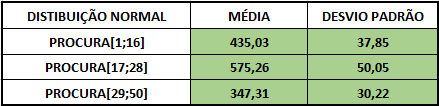
\includegraphics[scale=0.7]{distribuicao.png}
\caption{Valores da procura semanal para cada um dos 3 períodos}
\label{img:procura}
\end{figure}

De seguida, retiramos os valores possíveis para o prazo de entrega bem como as suas probabilidades respetivas.

\begin{figure}[H]
\centering
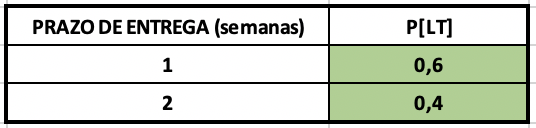
\includegraphics[scale=0.7]{prazo.png}
\caption{Valores das probabilidades dos prazos de entrega }
\label{img:prazo}
\end{figure}


Posteriormente foram retirados os valores referentes ao juro de existência (\textbf{i}) e ao valor unitário do artigo (\textbf{b}). Através destes valores calculamos automaticamente o valor do custo de posse (\textbf{C1}).

\begin{figure}[H]
\centering
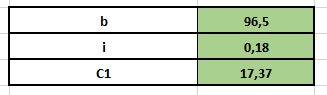
\includegraphics[scale=0.7]{Posse.png}
\caption{Custo de Posse}
\label{img:Posse}
\end{figure}

Logo após, calculamos o valor do custo de quebra (\textbf{C2}) através da fórmula: $$20+2*d1$$ sendo \textbf{d1} o último dígito do maior número mecanográfico de entre os elementos do grupo.
O custo de encomenda (\textbf{C3}) foi automaticamente retirado do enunciado tal como o ciclo de encomenda (\textbf{t}).

\begin{figure}[H]
\centering
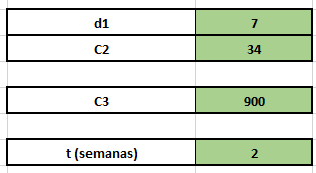
\includegraphics[scale=0.6]{c3c2t.png}
\caption{Custo de encomenda, Custo de quebra e Ciclo de encomenda}
\label{img:C3C2t}
\end{figure}


\subsection{Implementação}

Após a fase de análise dos dados disponíveis, começamos por construir um modelo de simulação que pudesse representar várias possibilidades de acontecimentos ao longo das 50 semanas (1 ano).

Para tal criamos uma grelha com 50 semanas e com as várias colunas apresentadas a seguir.

\begin{figure}[H]
\centering
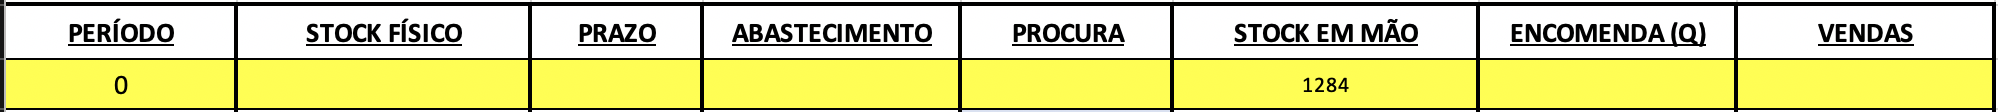
\includegraphics[scale=0.45]{grelha_simulacao.png}
\caption{Grelha de simulação com parâmetros a avaliar}
\label{img:grelha_sim}
\end{figure}

\subsubsection{Período}

O campo período é apenas uma coluna que indica o número da semana correspondente. As semanas marcadas com a célula a cinzento correspondem às semanas onde é realizada a decisão de encomendar ou não.

\begin{figure}[H]
\centering
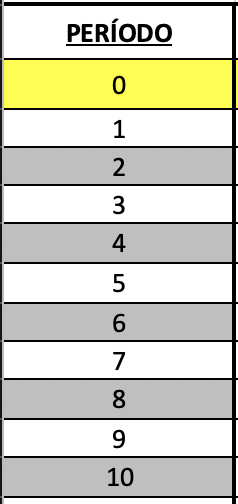
\includegraphics[scale=0.6]{periodo.png}
\caption{Coluna do período}
\label{img:periodo}
\end{figure}

Para o ano de 2019 estamos a considerar que as semanas estão compreendidas no intervalo \textbf{[1 , 50]}. Neste caso temos a semana 0 de forma a denotar que os campos não iniciam todos com valor 0 na primeira semana de 2019, mas que já vêm com alguns valores da última semana de 2018.


\subsubsection{Procura}

Uma vez que a procura foi retirada e calculada a partir do enunciado tal como é apresentado na secção \textbf{3.1}, para o nosso modelo de simulação adaptamos cada período a uma distribuição normal com a média e desvio padrão correspondestes aos mostrados na figura \ref{img:procura}.

No documento de excel cada período é representado com uma cor diferente.

\begin{figure}[H]
  \centering
  \begin{subfigure}[b]{0.3\linewidth}
    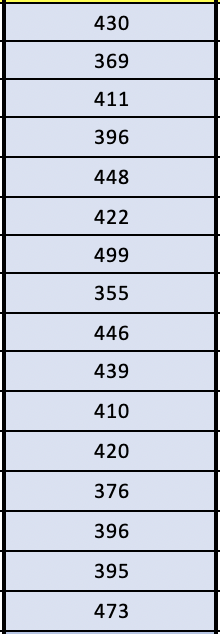
\includegraphics[scale = 0.6]{procura_p1.png}
    \caption{Procura no primeiro período.}
  \end{subfigure}
  \begin{subfigure}[b]{0.3\linewidth}
    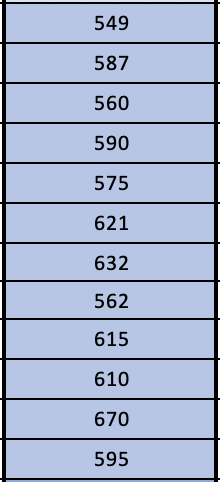
\includegraphics[scale=0.6]{procura_p2.png}
    \caption{Procura no segundo período}
  \end{subfigure}
  \begin{subfigure}[b]{0.3\linewidth}
    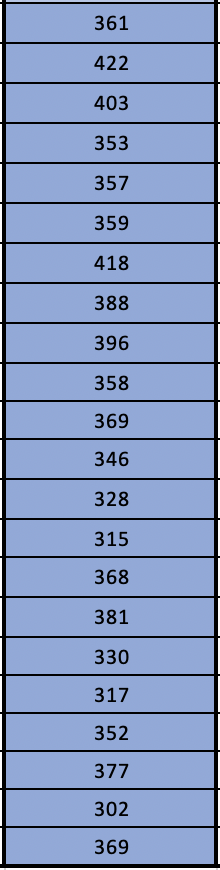
\includegraphics[scale=0.6]{procura_p3.png}
    \caption{Procura no terceiro período}
  \end{subfigure}
  \caption{Exemplo de valores de procura para os 3 períodos}
  \label{fig:proc}
\end{figure}

Para representar a procura como valores pertencentes a uma distribuição normal com uma dada média e desvio padrão no Excel utilizamos a fórmula:  $$ =INT(INV.NORMAL(ALEATORIO(); media ; desvio\ padrao)) $$

Desta forma é possível retirar uma valor inteiro que pertença à distribuição definida. Os valores da média e do desvio padrão correspondem aos valores anteriormente calculados.


\subsubsection{Prazo e Abastecimento}

Tal como especificado no enunciado e já visto na secção anterior existe um probabilidade duma encomenda chegar uma semana após o pedido da encomenda, e ainda a probabilidade de chegar duas semanas após o pedido de encomenda.

Considerando tal aspeto na ocorrência dum período após o pedido duma encomenda geramos um número aleatório entre 0 e 100, se este for menor que 40 então apresenta uma probabilidade de \textbf{0,4} (duas semanas), caso contrário apresenta uma probabilidade de \textbf{0,6} (uma semana).

A fórmula usada foi:  $$ =SE(ALEATORIOENTRE(0;100) < 40 ; 0,4 ; 0,6) $$

Os dois casos são ilustrados a seguir.

\begin{figure}[H]
  \centering
  \begin{subfigure}[b]{0.4\linewidth}
    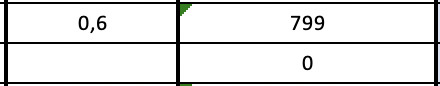
\includegraphics[scale = 0.6]{prazo_1sem.png}
    \caption{Prazo de entrega de uma semana}
  \end{subfigure}
  \begin{subfigure}[b]{0.5\linewidth}
    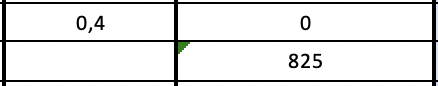
\includegraphics[scale=0.6]{prazo_2sem.png}
    \caption{Prazo de entrega de duas semanas}
  \end{subfigure}
  \caption{Exemplo de abastecimento consoante o prazo}
  \label{fig:praz}
\end{figure}

No caso de ser gerada uma probabilidade igual a \textbf{0,6} a quantidade é abastecida na primeira semana enquanto que na segunda nada é abastecido. No caso de ser gerada uma probabilidade igual a \textbf{0,4} a quantidade é abastecida na segunda semana enquanto que na primeira nada é abastecido.

A quantidade a abastecer tá ligada diretamente ao valor do pedido de encomenda realizado numa dada semana anterior.


\subsubsection{Stock Físico e Stock em Mão}

Para o nosso simulador consideramos o Stock Físico ligado diretamente ao Stock em Mão da semana anterior caso este seja maior ou igual a 0. Caso o Stock em Mão seja menor que 0, então o Stock Físico da semana seguinte não terá um valor negativo mas sim o valor 0. Tal tem que ser considerado uma vez que perante uma situação de quebra ocorre \textbf{Perda de Vendas}.

O Stock Físico da primeira semana é um valor que consideramos que seja o Stock em Mão da última semana de 2018. Calculamos este valor como sendo um número aleatório entre o primeiro par (S,s).

O Stock em Mão duma dada semana é calculado pela fórmula: $$ StockFisico - Procura + Abastecimento $$


\subsubsection{Encomenda (Q)}

No nosso simulador uma encomenda tem a possibilidade de ser feita de duas em duas semanas, por isso quando tal acontece o valor a encomendar será dado pelo algoritmo:

 $$ Q = SE(Stock\ em\ Mao\ <\ s\ ;\ SE(Stock\ em\ Mao\ <\ 0\ ;\ S\ ;\ S\ -\ Stock\ em\ Mao)\ ;\ 0 ) $$

 Uma vez que é necessário usar os valores (S,s) para determinar a quantidade a encomendar e como não temos apenas um par destes valores (tal será explicado em secções subsequentes), existem dois momentos críticos durante o ano nas duas transições de período.

\begin{figure}[H]
\centering
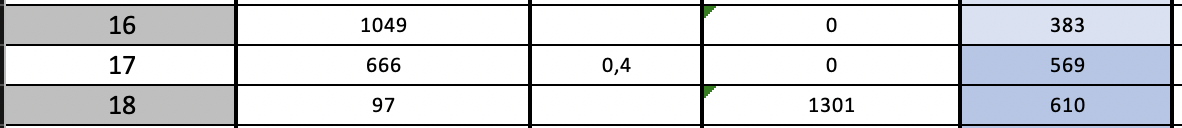
\includegraphics[scale=0.6]{periodo_critico.png}
\caption{Semana 16, 17 e 18}
\label{img:periodo_critico}
\end{figure}

Como se pode constatar da figura, a semana 16 é uma semana onde se vai encomendar algo. Ora ao encomendar na semana 16, a encomenda tanto pode chegar na semana 17 como na semana 18. Estas semanas já não pertencem ao mesmo período que a semana 16 pelo que se regem por valores diferentes de (S,s).

Desta forma a quantidade a encomendar na semana 16 tem que ter em consideração os valores (S,s) do período seguinte.

O nosso modelo de simulação encontra-se preparado para lidar com esta situação.


\subsubsection{Vendas}

Para saber quantas vendas foram realizadas numa dada semana é preciso ter em consideração a procura nessa semana bem como o Stock em Mão resultante. Desta forma utilizamos a seguinte forma para saber o número de vendas:

 $$ Vendas = SE(Stock\ em\ Mao >= 0\ ;\ Procura\ ;\ Procura\ +\ Stock\ em\ Mao) $$


\subsection{Execução}


\subsubsection{Valores analíticos para os pares (S,s)}

Após ter todo o simulador a construído, era preciso calcular os valores para (S,s), para antes de testar termos alguns valores de base, caso contrário teríamos de atribuir valores totalmente sem significado e avaliá-los.

Após algumas tentativas reparamos que os valores da procura estavam divididos em 3 períodos ([1,16], [17,28] e [29,50] ) pelo que determinar um par (S,s) para todo o ano poderia não ser de todo o mais ajustável.

\begin{figure}[H]
\centering
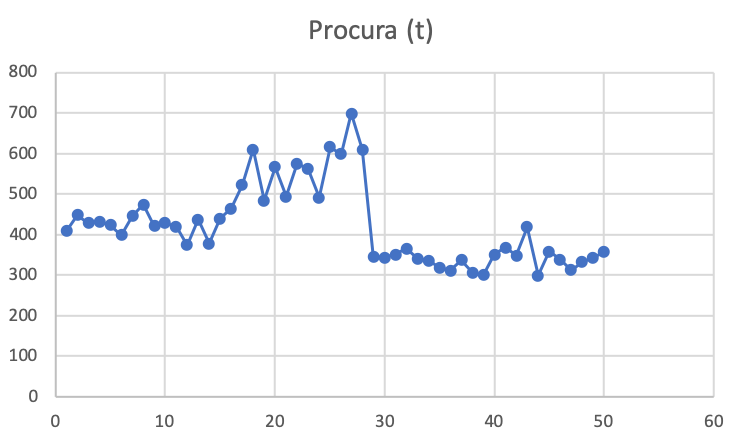
\includegraphics[scale=0.7]{grafico_procura.png}
\caption{Procura ao longo do ano}
\label{img:grafico_procura}
\end{figure}

Desta forma pensamos que se tivéssemos 3 pares de valores (S,s), um para cada diferente período poderíamos ajustar melhor as quantidades a encomendar em cada período, não regendo o terceiro período (procuras mais baixas) sobre o mesmo par (S,s) do segundo periodo (procuras mais altas), por exemplo.

Após decidirmos que teríamos 3 pares (S,s) tivemos que determinar analiticamente cada par. Aqui vamos apenas apresentar o cálculo do primeiro par, os restantes foram calculados tendo por base o mesmo raciocínio.

Para o primeiro período tivemos que que determinar a \textbf{probabilidade de quebra} que se resume na seguinte fórmula: 
 $$ P[DDPP > S][1,16] = \frac{1}{nº\ de\ ciclos\ no\ periodo} = \frac{1}{8} = 0.125$$
 
 Após calcular esta probabilidade seria necessário consultar a tabela da \textbf{Área da Distribuição Normal Standard, N(0,1)} para obter o \textbf{Z}. No Excel podemos obter o valor de Z utilizando a fórmula:
 $$ =ABS(INV.NORMP(probabilidade\ de\ quebra)) $$
 
 Para chegar a um valor de S é preciso ainda calcular $\mu_{DDPP}$ e o $\sigma_{DDPP}$, calculadas através das fórmulas:
 $$ INT(\ \mu_{DDPP}) = r \times (t + l) = 1479 $$
 $$ INT(\sigma_{DDPP}) = \sqrt{\sigma_{r}^2 \times (t + l)\ \ +\ \ r^2 \times \sigma_{l}^2} = 11 $$
 
 Tendo o \textbf{Z}, o \textbf{$\mu_{DDPP}$} e o \textbf{$\sigma_{DDPP}$} pode-se calcular o S através do teorema do limite central, através da fórmula:
 $$ S =  \mu_{DDPP}\ +\ Z \times \sigma_{DDPP} = 1491$$
 
 Para os outros períodos o procedimento foi exatamente o mesmo pelo que não é necessário demonstrar.
 
Falta ainda, agora que se descobriu o S, calcular a relação entre S e s que pode ser dada pela fórmula:
  $$ S = \sqrt{\frac{2 \times r \times C3}{C1}\ +\ s\ -\ r \times t} $$
Ora substituindo os valores já obtidos chegamos a uma relação que pode ser expressa por:
$$ s\ =\ S\ -\ 207,456 $$

Desta forma para o primeiro período deduzimos um par \textbf{(1491,1283)}, para o segundo período \textbf{(1967,1759)} e para o terceiro \textbf{(1193,985)}.


 \subsubsection{Stock médio}
 
 Após ter todo o simulador a funcionar corretamente o stock médio é simplesmente a \textbf{média inteira do Stock Físico}. Uma vez que existem valores aleatórios no simulador significa que o stock médio é uma medida que varia de tentativa para tentativa.
 
 \subsubsection{Quebras}
 
 De igual forma ao stock médio, uma vez tendo todos os valores disponíveis as quebras não se calculam através duma fórmula pré-concebida mas sim contando todas as vezes que o \textbf{Stock em Mão é menor que 0} nas 50 semanas. As quebras são também um parâmetro variável uma vez que dependem de valores aleatórios.
 
 \subsubsection{Custos}
  
 Tal como as duas medidas faladas anteriormente, também nos custos não podemos aplicar uma fórmula determinística uma vez que temos todos os dados ao nosso dispor e logo basta apenas calcular os custos tendo em conta o seguinte algoritmo:
 $$ Custos = (C1\ \times\ stock\ medio)\ +\ (C2\ \times\ nº\ de\ quebras)\ +\ (C3\ \times\ nº\ de\ encomendas) $$
 
 
 \subsubsection{Nível de Serviço}
 
 O nível de serviço duma tentativa é relacionado diretamente as quebras pela fórmula:
  $$ Nivel\ de\ Servico = 1 - \frac{nº\ de\ quebras}{nº\ de\ ciclos} $$
  
  
 \subsubsection{Lucro de Vendas}
 
 Para calcular o lucro das vendas basta somar todos os valores da coluna \textbf{VENDAS} e multiplicar pelo valor unitário do produto (120).
 
 \subsubsection{Número de artigos em quebra por ciclo}
  
 O número de artigos em quebra por ciclo relaciona diretamente a quantidade de artigos em quebra no Stock em Mão e o número de ciclos pela fórmula:
   $$ Artigos\ em\ quebra\ por\ ciclo\ = ABS(\frac{nº\ de\ artigos\ em\ quebra}{nº\ de\ ciclos}) $$






\section{Análise Estatística dos Resultados}

Após a construção, implementação e execução do modelo de simulação, foram realizados testes para encontrar a melhor abordagem a implementar na \textbf{ProLab}.

Tudo acerca da Simulação encontra-se na folha do Excel chamada \textbf{Simulador}, o que vamos abordar a seguir relaciona-se com os testes feitos ao simulador e os seus resultados estão na folha do Excel chamada \textbf{Testes}.

Tendo em conta os valores armazenados no simulador, foi calculada uma solução analítica para o \textbf{S(nível de referência)} e o \textbf{s(nível de encomenda)}, para cada um dos três intervalos de tempo do ano como já demonstrado anteriormente.

Os parâmetros que influenciaram as decisões foram a \textbf{média dos custos}, e a \textbf{média do nível de serviço}. A média dos custos, como é lógico, procuramos que fosse a \textbf{menor possível}, e a média do nível de serviço, impusemos que fosse \textbf{superior a 95\%}.

A partir da solução analítica foram realizadas 25 tentativas que deram origem a uma média de custos. No mesmo momento foram também guardados os valores que dão origem a uma média do nível de serviço.

Ora a partir dos valores obtidos para a solução analítica pensamos que ao baixar o \textbf{S} iríamos passar a encomendar menos e ter menos stock médio pelo que os custos iriam baixar, logo começamos por diminuir o \textbf{S} 5\% de cada vez.

Então diminuiu-se o nível de referência em 5\% e os custos diminuíram também. Colocando o mesmo nível em menos 10\% os custos diminuem, mas constatou-se que o nível de serviço baixou os 95\%. Desta forma, foi possível concluir que o melhor nível de referência é menos 5\% que a solução analítica.

Após obter um \textbf{S} com custos menores agora faltaria variar os valores de \textbf{s}. Enquanto o nível de serviço fosse superior a \textbf{95\%} variamos o valor de \textbf{s} de 5 em 5\% tal como anteriormente.

Paramos os testes quando diminuíamos \textbf{s} em 25\% porque foi possível reparar que a média do nível de serviço se encontrava abaixo dos 95\% tomado como referência.

Os testes realizados podem ser vistos na seguinte figura.

\begin{figure}[H]
\centering
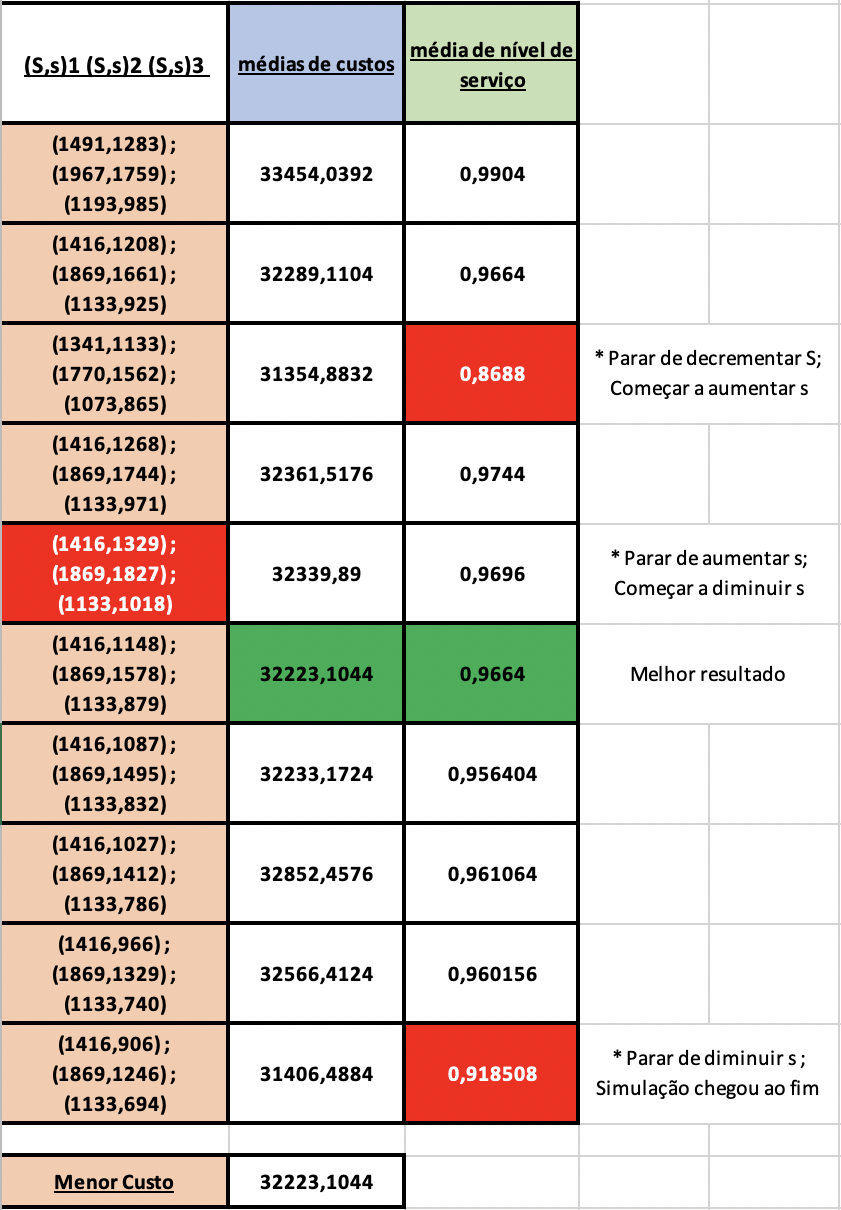
\includegraphics[scale=0.56]{testes.png}
\caption{Testes feitos ao simulador}
\label{img:testes}
\end{figure}

O melhor resultado encontrado foram os pares de valores para os períodos: \textbf{(1416,1148), (1869,1578), (1133,879)}. O custo relacionado com estes valores foi de \textbf{32223,1044}, com um nível de serviço \textbf{96,64\%}. Estes valores correspondem a um decréscimo de 5\% em ambos os valores analíticos calculados.


\section{Resultados e Conclusões}
\label{sec:conclusao}

Após todo o trabalho realizado o grupo aconselha a \textbf{ProLab} a implementar um método de considere 3 pares de valores (S,s), sendo que para o primeiro período entre as semanas 1 e 16, o par seja \textbf{(1416,1148)}, para o segundo período entre as semanas 17 e 28, o par seja \textbf{(1869,1578)} e para o terceiro período entre as semanas 29 e 50, o par seja \textbf{(1133,879)}.

Desta forma a empresa terá uns custos que irão rondar os \textbf{32223\euro} e apresentará um nível de serviço de aproximadamente \textbf{96,6\%}.

Para concluir, o grupo acha que os objetivos do trabalho, claramente explícitos no enunciado, foram cumpridos uma vez que apresentamos uma solução à empresa \textbf{ProLab} que achamos que esteja fundamentada com umas bases fortes de \textbf{Gestão de Stocks}.

\newpage

\begin{sidewaysfigure}
\section{Anexos}

\subsection{Folha Simulador}

\begin{figure}[H]
\centering
\makebox[\linewidth]{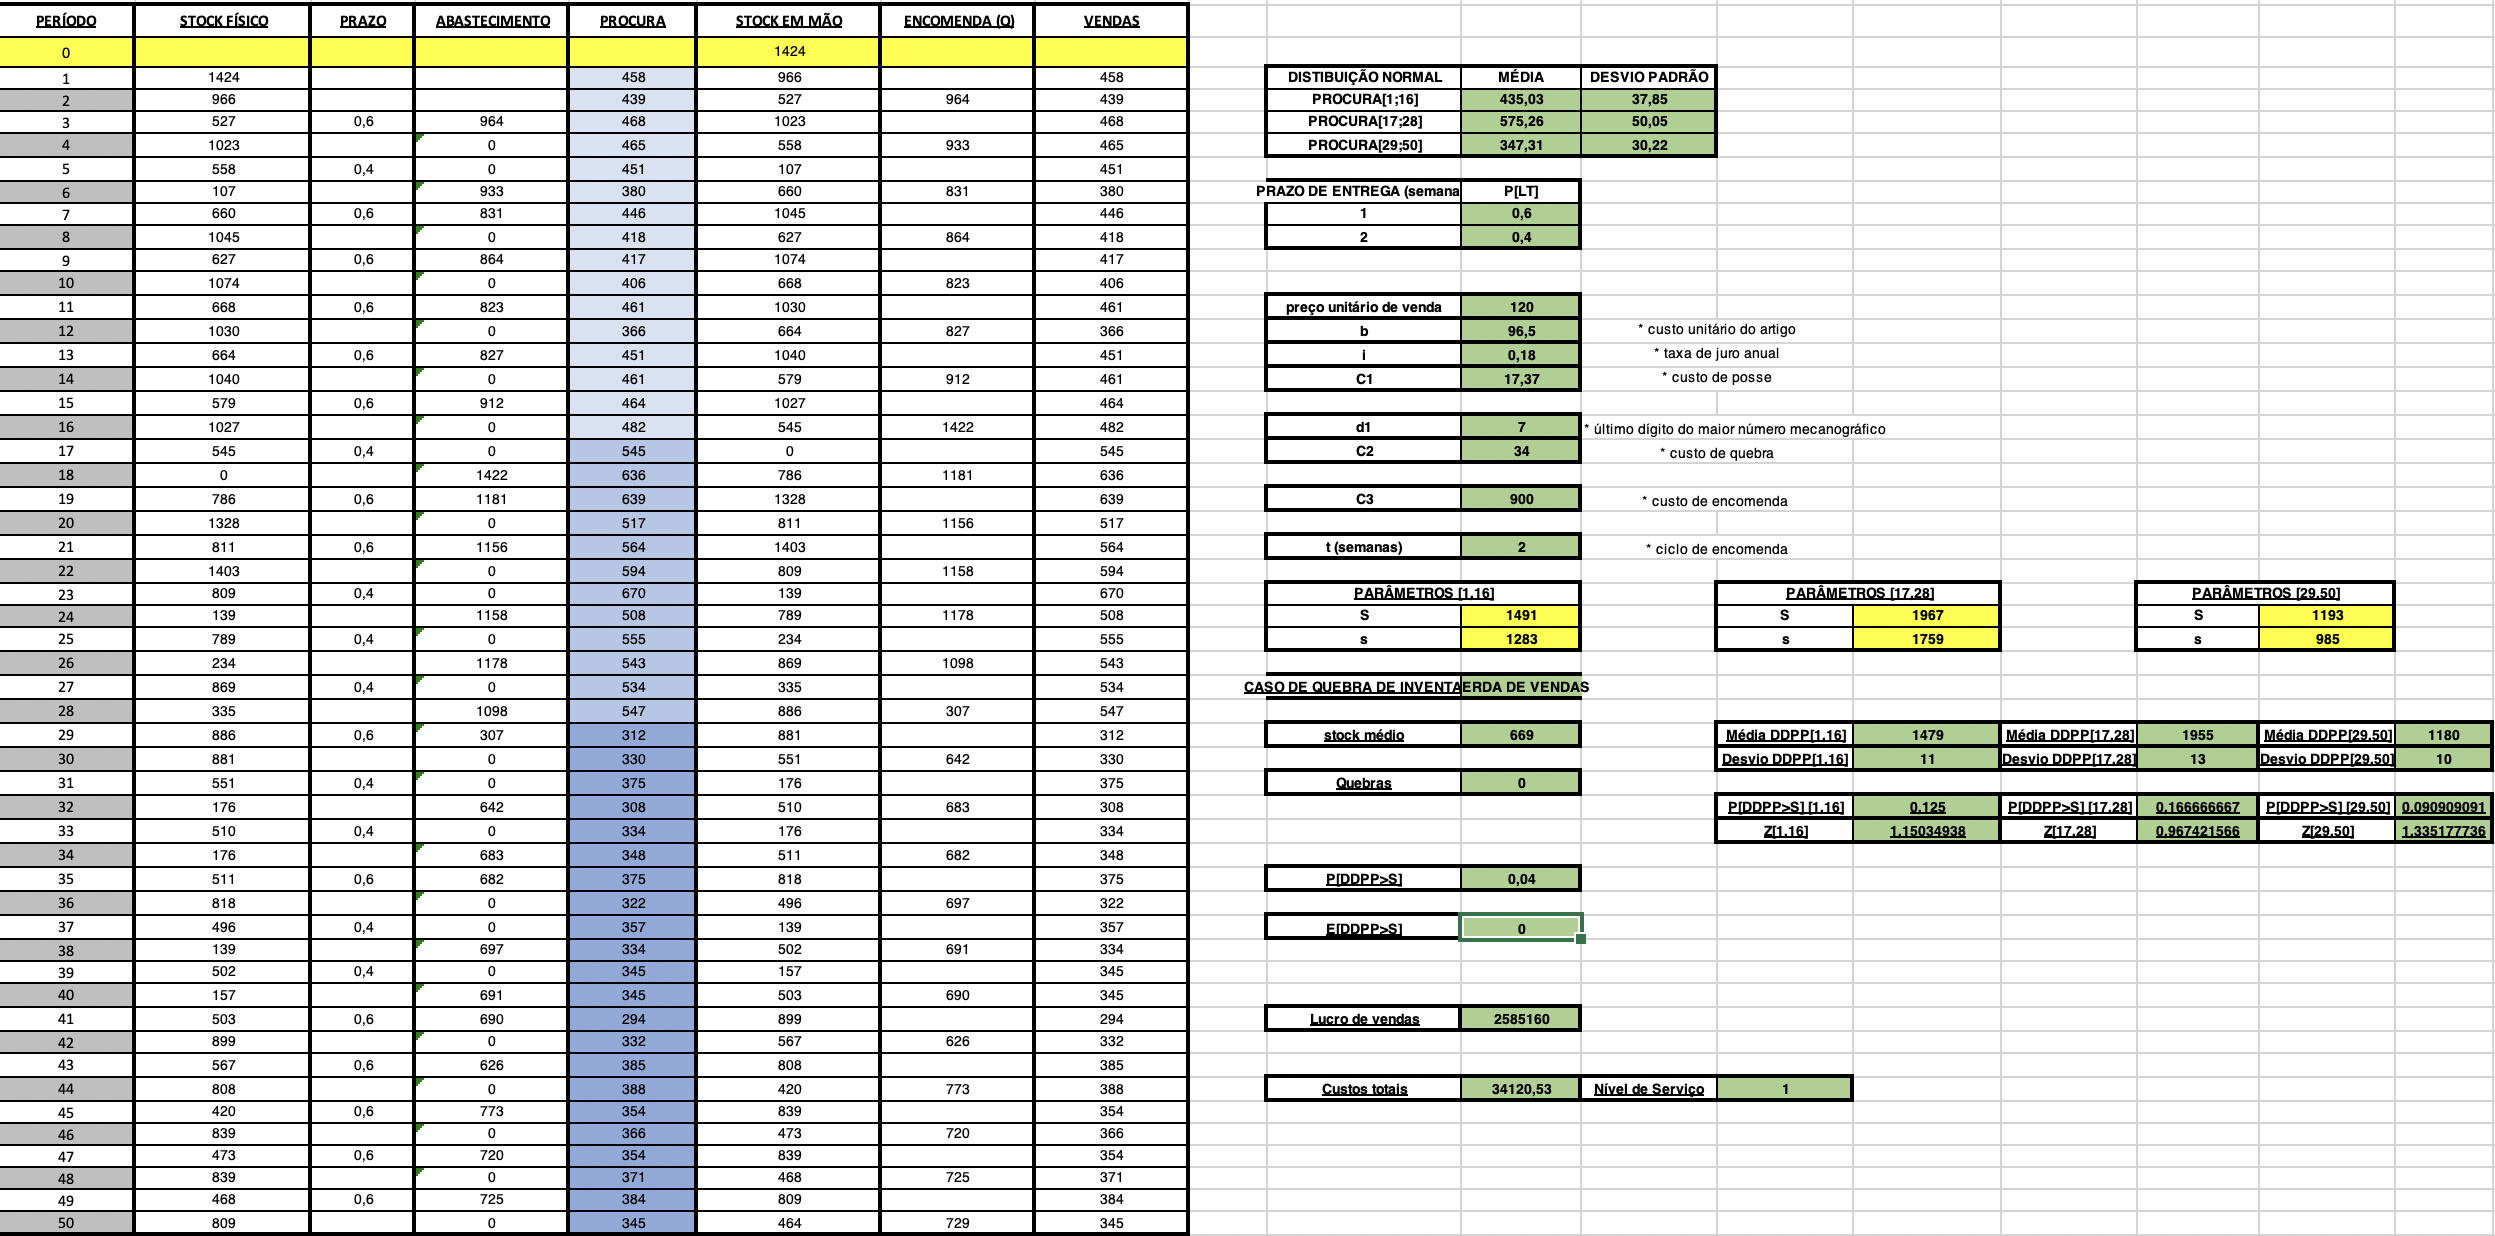
\includegraphics[scale=0.65]{Simulador.png}}
\caption{Folha Simulador do Excel}
\label{img:simulador}
\end{figure}
\end{sidewaysfigure}

\newpage

\begin{sidewaysfigure}
\subsection{Folha Testes}

\begin{figure}[H]
\centering
\makebox[\linewidth]{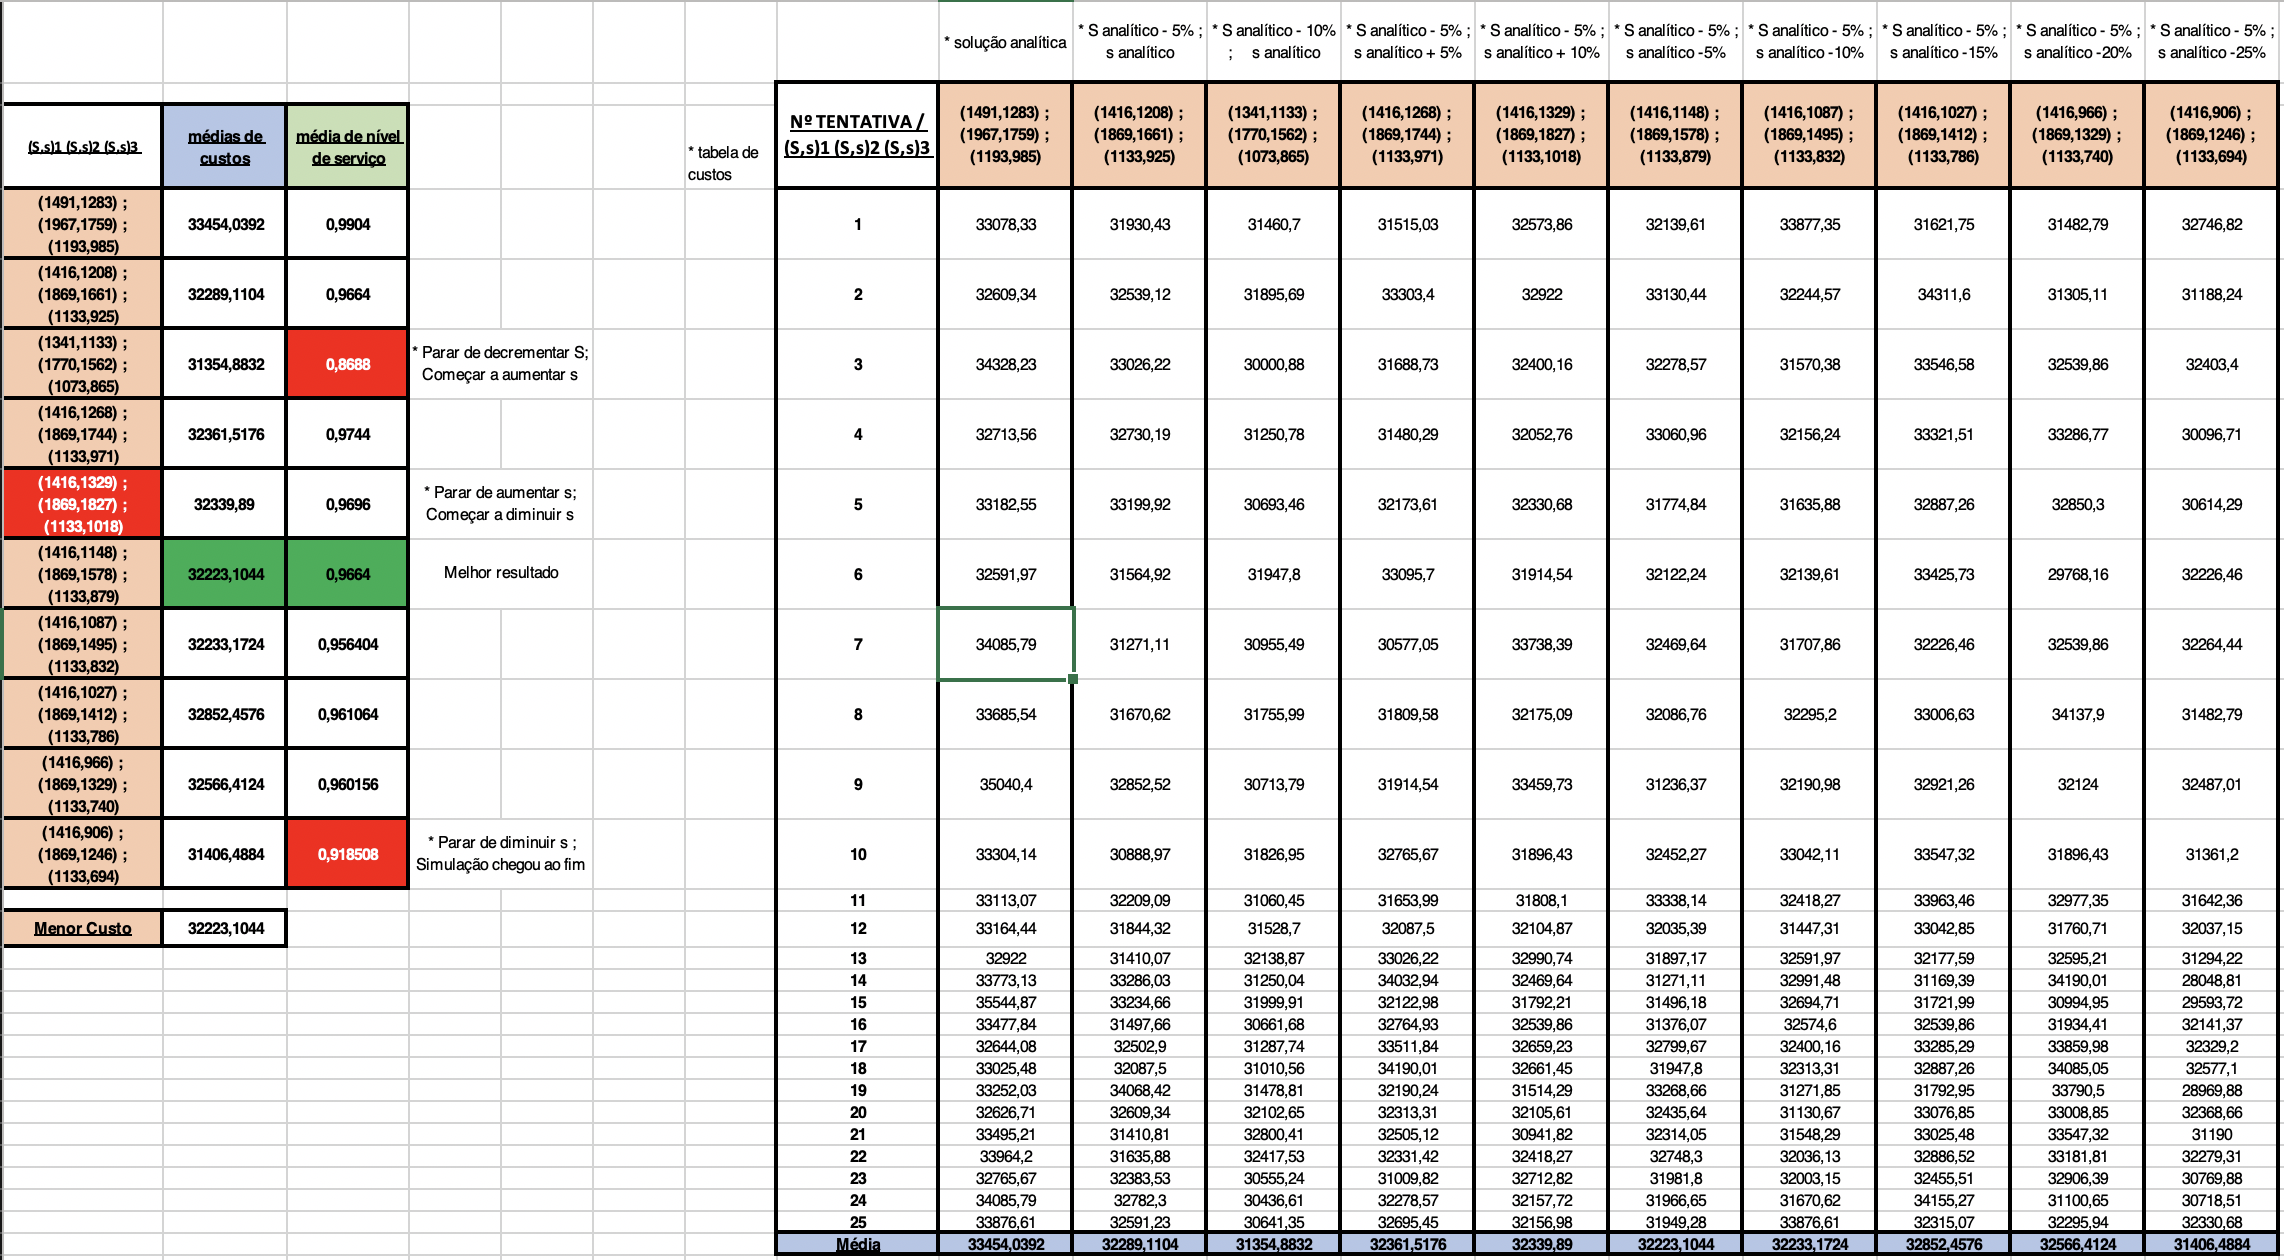
\includegraphics[scale=0.65]{Testes1.png}}
\caption{Folha Testes do Excel}
\label{img:testes1}
\end{figure}
\end{sidewaysfigure}

\newpage

\begin{sidewaysfigure}

\begin{figure}[H]
\centering
\makebox[\linewidth]{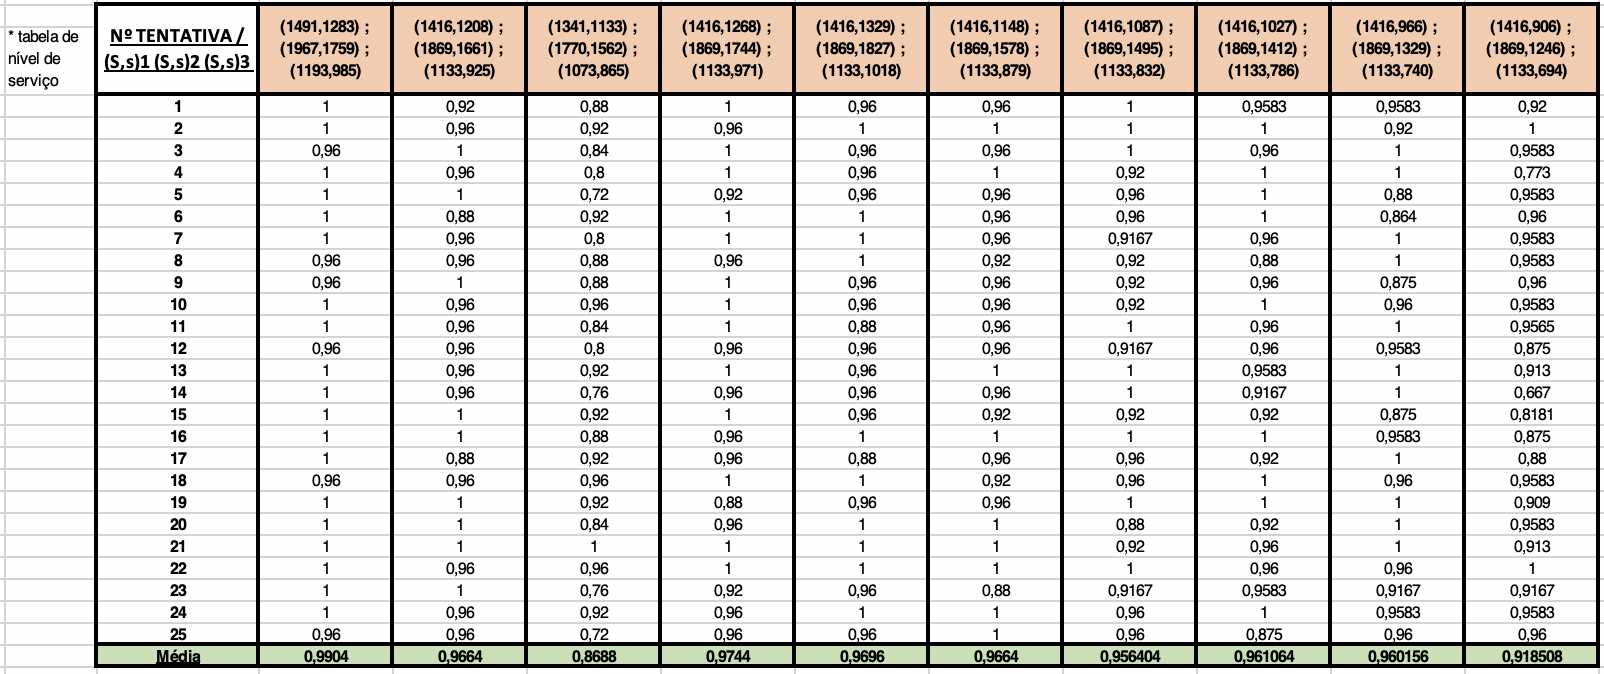
\includegraphics[scale=0.8]{Testes2.png}}
\caption{Folha Testes do Excel}
\label{img:testes2}
\end{figure}
\end{sidewaysfigure}



\end{document}
